\documentclass[parskip=full]{scrartcl}

\title{Pflichtenheft Energy-Schedules}

\date{22.5.2017}

\author{
	Rafael Quadbeck\\
	\and
	Daniel Bucher\\
	\and
	Christopher Greene\\
	\and
	Stefan Buzarnescu\\
	\and
	Max Scharfenberg\\
}

\usepackage{amsmath}
\usepackage{graphicx}
\usepackage[utf8]{inputenc}
\usepackage{enumitem}
\usepackage[german]{babel}

\begin{document}

	\pagenumbering{gobble}
	
	\maketitle
	
	\newpage
	
	\tableofcontents
	
	\listoffigures
	
	\listoftables
	
	\newpage
	
	\pagenumbering{arabic}
	
	\section{Zielbestimmung}
		Das Produkt soll Schedules einlesen, übersichtlich anzeigen können.\\ Zusätzlich soll die Bearbeitung von Schedules möglich sein und die Daten eines Jobs sollen angezeigt werden können.\\ Außerdem soll die Schedule gespeichert werden und als Bild exportiert werden können.\\
		\subsection{Musskriterien}
			Einlesen von Schedules\\
			Schedule darstellen\\
			Anzeigen von Informationen der einzelnen Blöcke\\
			Ordnen der Blöcke\\
			Speichern der Schedule\\
			Ändern der Dauer eines Blocks\\
			Ändern der Höhe eines Blocks\\
			Exportieren als Bild\\
			Gesamtverbrauch = Höhe der Blöcke\\
		\subsection{Wunschkriterien}
			Nur die Skyline anzeigen\\
			Kurve des Energieverbrauchs (maximal)\\
			Darstellung unterschiedlicher Ressourcen\\
			Auflistung aller Prozesse\\
			Unterschiedlicher Höhen innerhalb eines Blockes\\
			Neufärbung bei Veränderung eines Blockes\\
			Färben von Blöcken\\
		\subsection{Abgrenzungskriterien}
			Keine automatische Speicherung/Einlesung der Schedules\\
			Kein Vergleich / Interaktion zwischen Schedules\\
			Kein simultanes Darstellen mehrerer Ressourcen\\
			Keine Ressourcenproduktion\\
			Kein Erstellen und Löschen von Prozessen\\
			
			
	\section{Produkteinsatz}
		Das Produkt dient zur Visualisierung und Bearbeitung von Energie-Schedules\\
		Es erleichtert die Übersicht und Organisation von Ressourcen innerhalb eines Smart-Grids\\
		\subsection{Anwendungsbereiche}
			Erforschung von Energie-Schedules in Smart-Grids\\
			
		\subsection{Zielgruppen}
			Benutzer von Energy-Schedules mit ...format\\
			
		\subsection{Betriebsbedingungen}
			Forschungsumgebung aktuelles Java Runtime Environment muss installiert sein\\
			
	\section{Produktumgebung}
		\subsection{Software}
			Microsoft Windows, MAC OSX, Linux
		\subsection{Hardware}
		Computer\\
	\section{Funktionale Anforderungen}
		\subsection{Muss-Funktionalität}
			
			
			\textbf{/F10/} Darstellen der Blöcke\\\\\\
			\textbf{/F20/} Verändern der Anfangszeit\\\\
			\textbf{/F20/} Verändern der Endzeit\\\\
			\textbf{/F20/} Bearbeiten der Länge\\\\
			\textbf{/F20/} Bearbeiten der Höhe\\\\
			\textbf{/F20/} Importieren einer Schedule\\\\
			\textbf{/F20/} Speichern einer Schedule\\\\
			\textbf{/F20/} Automatische Anordnung der Blöcke in der Höhe\\\\
			\textbf{/F20/} Informationen über die Blöcke anzeigen\\\\
			\textbf{/F20/} Mittels Mausinteraktion Jobs verschieben\\\\
			\textbf{/F20/} Anzeige als Bild exportieren\\\\				
			\textbf{/F20/} Ein Job wird als Block dargestellt\\\\
		\textbf{/F20/} Jobs werden durch ihre eindeutige ID gekennzeichnet\\\\
		\textbf{/F20/} Name/ID werden im Block angezeigt\\\\			
		\textbf{/F20/} Bei ungespeicherten Veränderungen einer Schedule wird bei Schließen des Programms gefragt, ob gespeichert werden soll\\\\			
		
		\subsection{Optionale Funktionalität}
			\textbf{/F20/} Automatische Färbung der Blöcke\\\\
			
			\textbf{/F30/} ...\\\\
	
				
		\subsection{...}
		
	\section{Produktdaten}
		\subsection{Schedule-Daten}
			Prozessname, Anfangszeit, Endzeit, Länge, Leistung
			
	\section{Nichtfunktionale 		Anforderungen}
		
		
			\textbf{/NF10/} Es müssen 10.000 Blöcke verwaltet werden können\\\\
			
			\textbf{/NF20/} Nach einer Stunde begeht der Nutzer höchstens einen Fehler pro Stunde\\\\
			Muss objektorientiert sein\\
			Nach dem Wasserfallmodell\\
			Softwarebib müssen frei und akademische Lizenz\\
			Soll schedule in ... anzeigen können\\
			Änderungen sollen in unter 200 ms angezeigt werden\\
			Neufärbung soll unter 2 Sekunden dauern\\
			
			
			
	\section{Globale Testfälle}
		\subsection{Funktionssequenzen}
			
			
				\textbf{/T10/} Schedule einlesen, Informationen abfragen, Schedule ändern, speichern\\\\
				\textbf{/T20/} Färbung\\\\
				\textbf{/T20/} Anfangszeit ändern\\\\
				\textbf{/T20/} Schedule einlesen, ändern, speichern, laden\\\\
				\textbf{/T20/} Illegale Datei einlesen\\\\
				\textbf{/T10/} Programm starten
				\textbf{/T10/} Schedule einlesen
				\textbf{/T10/} Einordnung
				\textbf{/T10/} Neufärbung
				\textbf{/T10/} Wird gezeichnet?
				\textbf{/T10/} Gültigkeit der Zeichnung
				\textbf{/T10/} Verschiebung
				\textbf{/T10/} Zeitveränderung
				\textbf{/T10/} Ressourcenveränderung
				\textbf{/T10/} Bild exportieren
				\textbf{/T10/} Programm beenden
				\textbf{/T10/} Was passiert bei Absturz?
				\textbf{/T10/} Grenzwerte testen
				
				
				
		\subsection{Datenkonsistenzen}
		
	\section{Systemmodelle}
		\subsection{Szenarien}
		Szenario 1: Fredericka ist Besitzerin eines Smart-Homes. Sie öffnet das Programm um ihren Energieverbrauch einzusehen. Sie sieht, dass er viel zu hoch ist. Darum verlegt sie die Waschmaschine auf Mittag, wo die Sonne scheint. Außerdem exportiert sie das Bild und hängt es an ihre Waschmaschine. Alle sind froh. Das Ende.\\\\
		Szenario 2: Rüdiger arbeitet in einer Fabrik. Die letzt Stromrechnung hat ihm die Sprache verschlagen. Er möchte der Sache auf den Grund gehen. Von IT-Spezialisten aus der ganzen Welt, wird ihm das Programm empfohlen. Er holt es sich sofort, und startet es. Er sieht nun den Energieverbrauch der Geräte in der Fabrik in einer außerordentlich schönen Darstellung. Er bemerkt, dass ein Gerät einen extrem hohen Verbrauch hat. Er klickt auf den sehr hohen Balken. Er identifiziert den Job anhand der eindeutigen ID. Nun schaut er die Maschine an. Er tauscht das defekte Teil aus. 
		Szenario 3:
		\subsection{Anwendungsfälle}
		
		Name Schedule einlesen, bearbeiten und als Bild exportieren\\
		Teilnehmende Akteure Benutzer
		
		Eingangsbedingung Es besteht eine Energy-Schedule in passendem Format
		Ereignisfluss Benutzer startet das Program\\
		Benutzer schauet die Darstellung an\\
		Benutzer verändert Lage eines Blocks\\
		Benutzer speichert die Schedule\\
		Benutzer beendet das Program\\
		
		Name Schedule einlesen, anschauen, als Bild exportieren\\
		Teilnehmende Akteure Benutzer\\
		Eingangsbedingung Es besteht eine Energy-Schedule in passendem Format\\
		Ereignisfluss Benutzer startet das Program\\
		Benutzer schaut Grafik an\\
		Benutzer exportiert das Bild\\
		Benutzer beendet das Program\\
			\begin{figure}[h!]
			
				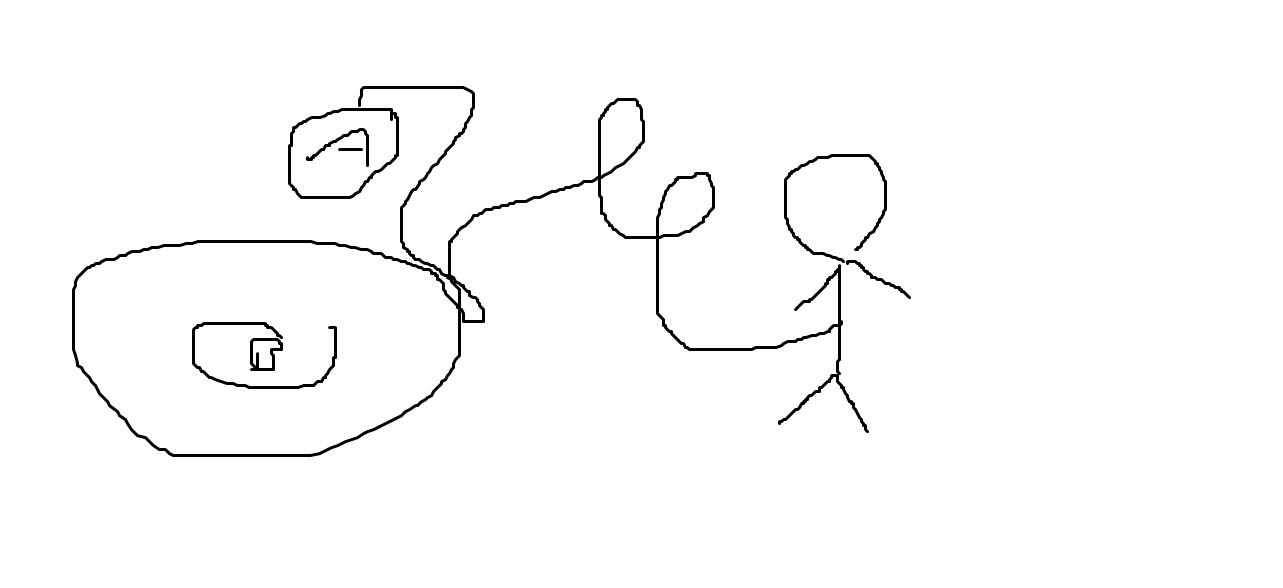
\includegraphics[width=\linewidth]{img/usecase1.jpg}
				\caption{User does ... something?}
				\label{fig:uc1}
				
			\end{figure}
			
			Abbildung \ref{fig:uc1} zeigt unseren ersten Anwendungsfall.
			
		\subsection{Benutzerschnittstelle}


			\textbf{/B10/} Soll mit Maus bedient werden.\\\\
			
			\textbf{/B20/} Steuerung ohne Maus soll auch möglich sein\\\\
			
			
	\section{Glossar}
	
\end{document}